\documentclass{standalone}
\usepackage{tikz}
\usetikzlibrary{patterns, positioning}

\begin{document}
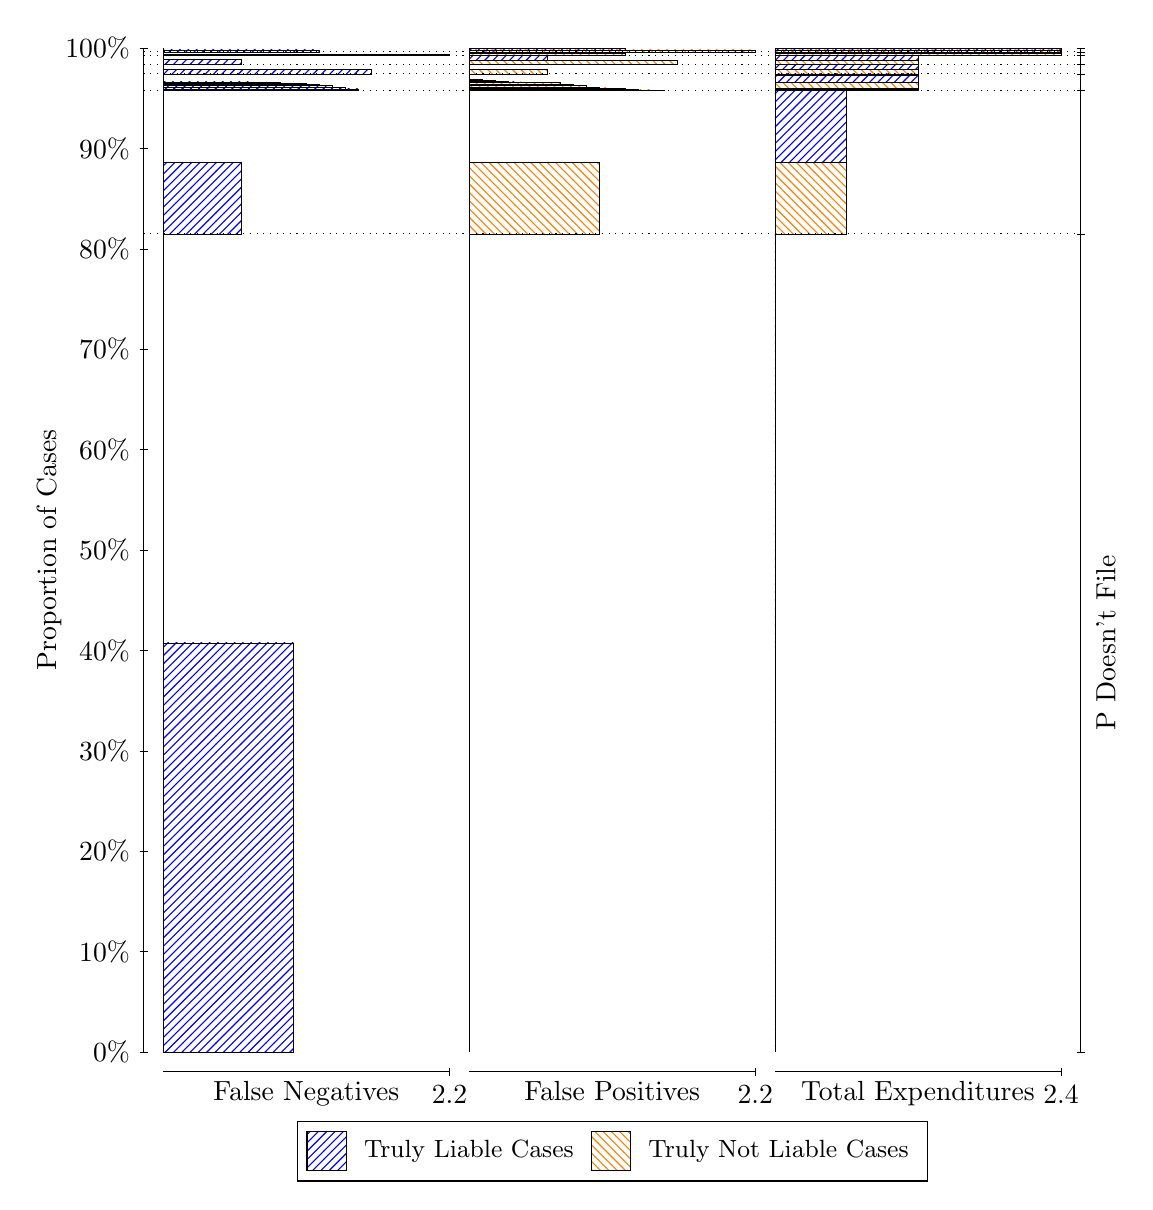
\begin{tikzpicture}
\draw[black, very thin] (1.5,1.75) -- (1.5,14.5);
\node[rotate=90, anchor=center] at (0.3, 8.125) {Proportion of Cases};
\draw[black, very thin] (1.45,1.75) -- (1.55,1.75);
\node[anchor=east] at (1.45, 1.75) {0\%};
\draw[black, very thin] (1.45,3.025) -- (1.55,3.025);
\node[anchor=east] at (1.45, 3.025) {10\%};
\draw[black, very thin] (1.45,4.3) -- (1.55,4.3);
\node[anchor=east] at (1.45, 4.3) {20\%};
\draw[black, very thin] (1.45,5.575) -- (1.55,5.575);
\node[anchor=east] at (1.45, 5.575) {30\%};
\draw[black, very thin] (1.45,6.85) -- (1.55,6.85);
\node[anchor=east] at (1.45, 6.85) {40\%};
\draw[black, very thin] (1.45,8.125) -- (1.55,8.125);
\node[anchor=east] at (1.45, 8.125) {50\%};
\draw[black, very thin] (1.45,9.4) -- (1.55,9.4);
\node[anchor=east] at (1.45, 9.4) {60\%};
\draw[black, very thin] (1.45,10.675) -- (1.55,10.675);
\node[anchor=east] at (1.45, 10.675) {70\%};
\draw[black, very thin] (1.45,11.95) -- (1.55,11.95);
\node[anchor=east] at (1.45, 11.95) {80\%};
\draw[black, very thin] (1.45,13.225) -- (1.55,13.225);
\node[anchor=east] at (1.45, 13.225) {90\%};
\draw[black, very thin] (1.45,14.5) -- (1.55,14.5);
\node[anchor=east] at (1.45, 14.5) {100\%};

\draw[black, very thin] (13.4,1.75) -- (13.4,14.5);
\draw[black, very thin] (13.35,1.75) -- (13.45,1.75);
\node[anchor=west] at (13.35, 1.75) {};
\draw[black, very thin] (13.35,12.14) -- (13.45,12.14);
\node[anchor=west] at (13.35, 12.14) {};
\draw[black, very thin] (13.35,13.961) -- (13.45,13.961);
\node[anchor=west] at (13.35, 13.961) {};
\draw[black, very thin] (13.35,14.172) -- (13.45,14.172);
\node[anchor=west] at (13.35, 14.172) {};
\draw[black, very thin] (13.35,14.288) -- (13.45,14.288);
\node[anchor=west] at (13.35, 14.288) {};
\draw[black, very thin] (13.35,14.403) -- (13.45,14.403);
\node[anchor=west] at (13.35, 14.403) {};
\draw[black, very thin] (13.35,14.452) -- (13.45,14.452);
\node[anchor=west] at (13.35, 14.452) {};
\draw[black, very thin] (13.35,14.5) -- (13.45,14.5);
\node[anchor=west] at (13.35, 14.5) {};

\draw[black, very thin, pattern color=blue, pattern=north east lines] (1.75,1.75) rectangle (3.4015,6.9448);
\draw[black, very thin, pattern color=orange, pattern=north west lines] (1.75,6.9448) rectangle (1.75,12.14);
\draw[black, very thin, pattern color=blue, pattern=north east lines] (1.75,12.14) rectangle (2.7409,13.048);
\draw[black, very thin, pattern color=orange, pattern=north west lines] (1.75,13.048) rectangle (1.75,13.961);
\draw[black, very thin, pattern color=blue, pattern=north east lines] (1.75,13.961) rectangle (4.2273,13.981);
\draw[black, very thin, pattern color=blue, pattern=north east lines] (1.75,13.981) rectangle (4.0621,13.999);
\draw[black, very thin, pattern color=blue, pattern=north east lines] (1.75,13.999) rectangle (3.897,14.026);
\draw[black, very thin, pattern color=blue, pattern=north east lines] (1.75,14.026) rectangle (3.7318,14.034);
\draw[black, very thin, pattern color=blue, pattern=north east lines] (1.75,14.034) rectangle (3.5667,14.047);
\draw[black, very thin, pattern color=blue, pattern=north east lines] (1.75,14.047) rectangle (3.4015,14.055);
\draw[black, very thin, pattern color=blue, pattern=north east lines] (1.75,14.055) rectangle (3.2364,14.063);
\draw[black, very thin, pattern color=blue, pattern=north east lines] (1.75,14.063) rectangle (3.0712,14.066);
\draw[black, very thin, pattern color=blue, pattern=north east lines] (1.75,14.066) rectangle (2.9061,14.07);
\draw[black, very thin, pattern color=orange, pattern=north west lines] (1.75,14.07) rectangle (1.75,14.172);
\draw[black, very thin, pattern color=blue, pattern=north east lines] (1.75,14.172) rectangle (4.3924,14.228);
\draw[black, very thin, pattern color=orange, pattern=north west lines] (1.75,14.228) rectangle (1.75,14.288);
\draw[black, very thin, pattern color=blue, pattern=north east lines] (1.75,14.288) rectangle (2.7409,14.352);
\draw[black, very thin, pattern color=orange, pattern=north west lines] (1.75,14.352) rectangle (1.75,14.403);
\draw[black, very thin, pattern color=blue, pattern=north east lines] (1.75,14.403) rectangle (5.3833,14.423);
\draw[black, very thin, pattern color=orange, pattern=north west lines] (1.75,14.423) rectangle (1.75,14.452);
\draw[black, very thin, pattern color=blue, pattern=north east lines] (1.75,14.452) rectangle (3.7318,14.476);
\draw[black, very thin, pattern color=orange, pattern=north west lines] (1.75,14.476) rectangle (1.75,14.5);
\draw[black, very thin, pattern color=orange, pattern=north west lines] (5.6333,1.75) rectangle (5.6333,6.9448);
\draw[black, very thin, pattern color=blue, pattern=north east lines] (5.6333,6.9448) rectangle (5.6333,12.14);
\draw[black, very thin, pattern color=orange, pattern=north west lines] (5.6333,12.14) rectangle (7.2848,13.052);
\draw[black, very thin, pattern color=blue, pattern=north east lines] (5.6333,13.052) rectangle (5.6333,13.961);
\draw[black, very thin, pattern color=orange, pattern=north west lines] (5.6333,13.961) rectangle (8.1106,13.964);
\draw[black, very thin, pattern color=orange, pattern=north west lines] (5.6333,13.964) rectangle (7.9455,13.968);
\draw[black, very thin, pattern color=orange, pattern=north west lines] (5.6333,13.968) rectangle (7.7803,13.975);
\draw[black, very thin, pattern color=orange, pattern=north west lines] (5.6333,13.975) rectangle (7.6152,13.983);
\draw[black, very thin, pattern color=orange, pattern=north west lines] (5.6333,13.983) rectangle (7.45,13.995);
\draw[black, very thin, pattern color=orange, pattern=north west lines] (5.6333,13.995) rectangle (7.2848,14.003);
\draw[black, very thin, pattern color=orange, pattern=north west lines] (5.6333,14.003) rectangle (7.1197,14.025);
\draw[black, very thin, pattern color=orange, pattern=north west lines] (5.6333,14.025) rectangle (6.9545,14.04);
\draw[black, very thin, pattern color=orange, pattern=north west lines] (5.6333,14.04) rectangle (6.7894,14.063);
\draw[black, very thin, pattern color=blue, pattern=north east lines] (5.6333,14.063) rectangle (6.4591,14.067);
\draw[black, very thin, pattern color=blue, pattern=north east lines] (5.6333,14.067) rectangle (6.2939,14.07);
\draw[black, very thin, pattern color=blue, pattern=north east lines] (5.6333,14.07) rectangle (6.1288,14.078);
\draw[black, very thin, pattern color=blue, pattern=north east lines] (5.6333,14.078) rectangle (5.9636,14.086);
\draw[black, very thin, pattern color=blue, pattern=north east lines] (5.6333,14.086) rectangle (5.7985,14.099);
\draw[black, very thin, pattern color=blue, pattern=north east lines] (5.6333,14.099) rectangle (5.6333,14.172);
\draw[black, very thin, pattern color=orange, pattern=north west lines] (5.6333,14.172) rectangle (6.6242,14.233);
\draw[black, very thin, pattern color=blue, pattern=north east lines] (5.6333,14.233) rectangle (5.6333,14.288);
\draw[black, very thin, pattern color=orange, pattern=north west lines] (5.6333,14.288) rectangle (8.2758,14.339);
\draw[black, very thin, pattern color=blue, pattern=north east lines] (5.6333,14.339) rectangle (6.6242,14.403);
\draw[black, very thin, pattern color=orange, pattern=north west lines] (5.6333,14.403) rectangle (7.6152,14.432);
\draw[black, very thin, pattern color=blue, pattern=north east lines] (5.6333,14.432) rectangle (5.9636,14.452);
\draw[black, very thin, pattern color=orange, pattern=north west lines] (5.6333,14.452) rectangle (9.2667,14.476);
\draw[black, very thin, pattern color=blue, pattern=north east lines] (5.6333,14.476) rectangle (7.6152,14.5);
\draw[black, very thin, pattern color=orange, pattern=north west lines] (9.5167,1.75) rectangle (9.5167,6.9448);
\draw[black, very thin, pattern color=blue, pattern=north east lines] (9.5167,6.9448) rectangle (9.5167,12.14);
\draw[black, very thin, pattern color=orange, pattern=north west lines] (9.5167,12.14) rectangle (10.425,13.052);
\draw[black, very thin, pattern color=blue, pattern=north east lines] (9.5167,13.052) rectangle (10.425,13.961);
\draw[black, very thin, pattern color=orange, pattern=north west lines] (9.5167,13.961) rectangle (11.333,13.973);
\draw[black, very thin, pattern color=blue, pattern=north east lines] (9.5167,13.973) rectangle (11.333,13.986);
\draw[black, very thin, pattern color=orange, pattern=north west lines] (9.5167,13.986) rectangle (11.333,14.066);
\draw[black, very thin, pattern color=blue, pattern=north east lines] (9.5167,14.066) rectangle (11.333,14.151);
\draw[black, very thin, pattern color=orange, pattern=north west lines] (9.5167,14.151) rectangle (11.333,14.161);
\draw[black, very thin, pattern color=blue, pattern=north east lines] (9.5167,14.161) rectangle (11.333,14.172);
\draw[black, very thin, pattern color=orange, pattern=north west lines] (9.5167,14.172) rectangle (11.333,14.233);
\draw[black, very thin, pattern color=blue, pattern=north east lines] (9.5167,14.233) rectangle (11.333,14.288);
\draw[black, very thin, pattern color=orange, pattern=north west lines] (9.5167,14.288) rectangle (11.333,14.339);
\draw[black, very thin, pattern color=blue, pattern=north east lines] (9.5167,14.339) rectangle (11.333,14.403);
\draw[black, very thin, pattern color=orange, pattern=north west lines] (9.5167,14.403) rectangle (13.15,14.432);
\draw[black, very thin, pattern color=blue, pattern=north east lines] (9.5167,14.432) rectangle (13.15,14.452);
\draw[black, very thin, pattern color=orange, pattern=north west lines] (9.5167,14.452) rectangle (13.15,14.476);
\draw[black, very thin, pattern color=blue, pattern=north east lines] (9.5167,14.476) rectangle (13.15,14.5);
\draw[black, dotted] (1.5,12.14) -- (13.4,12.14);
\draw[black, dotted] (1.5,13.961) -- (13.4,13.961);
\draw[black, dotted] (1.5,14.172) -- (13.4,14.172);
\draw[black, dotted] (1.5,14.288) -- (13.4,14.288);
\draw[black, dotted] (1.5,14.403) -- (13.4,14.403);
\draw[black, dotted] (1.5,14.452) -- (13.4,14.452);
\draw[black, very thin] (1.75,1.5) -- (5.3833,1.5);
\node[anchor=north] at (3.5667, 1.5) {False Negatives};
\draw[black, very thin] (5.3833,1.45) -- (5.3833,1.55);
\node[anchor=north] at (5.3833, 1.45) {2.2};

\draw[black, very thin] (5.6333,1.5) -- (9.2667,1.5);
\node[anchor=north] at (7.45, 1.5) {False Positives};
\draw[black, very thin] (9.2667,1.45) -- (9.2667,1.55);
\node[anchor=north] at (9.2667, 1.45) {2.2};

\draw[black, very thin] (9.5167,1.5) -- (13.15,1.5);
\node[anchor=north] at (11.333, 1.5) {Total Expenditures};
\draw[black, very thin] (13.15,1.45) -- (13.15,1.55);
\node[anchor=north] at (13.15, 1.45) {2.4};

\node[black, centered, rotate=90] at (13.72, 6.9448) {P Doesn't File};







\draw (7.449999999999999,1.5) node[draw=none] (baseCoordinate) {};
\begin{scope}[align=center]
        \matrix[scale=0.5, draw=black, below=0.5cm of baseCoordinate, nodes={draw}, column sep=0.1cm]{
            \node[rectangle, draw, minimum width=0.5cm, minimum height=0.5cm, pattern=north east lines, pattern color=blue] {}; &
            \node[draw=none, font=\small] (B) {Truly Liable Cases}; &
            \node[rectangle, draw, minimum width=0.5cm, minimum height=0.5cm, pattern=north west lines, pattern color=orange] {}; &
            \node[draw=none, font=\small] (B) {Truly Not Liable Cases}; \\
            };
\end{scope}

\end{tikzpicture}
\end{document}